\documentclass[aspectratio=169,11pt]{beamer}
\usetheme{Boadilla}
\usecolortheme{seahorse}
\usepackage{booktabs,amsmath}
\definecolor{navy}{RGB}{26,53,77}
\setbeamercolor{structure}{fg=navy}
\setbeamercolor{frametitle}{fg=navy,bg=white}
\setbeamertemplate{navigation symbols}{}
\setbeamertemplate{footline}[frame number]
\graphicspath{{../report/figures/}}
\newcommand{\figcaption}[1]{\par\vspace{2pt}{\scriptsize #1}}
\title{Kidney Stone Segmentation Using Deep Learning}
\subtitle{Controlled replication and attention skip-gate study}
\author{[ALL MEMBER NAMES AND ROLL NUMBERS REQUIRED]}
\institute{22AIE437 -- Medical Image Processing\\Amrita School of Artificial Intelligence\\Group: [NAME/NUMBER REQUIRED]}
\date{13 October 2026}
\begin{document}

\begin{frame}{1. Problem, motivation and project team}
\begin{columns}[T]
\column{.62\textwidth}
{\Large Kidney stone segmentation}\par\medskip
\begin{itemize}
\item Delineate annotated stone pixels in axial CT exports.
\item Pixel masks retain location and extent for image analysis.
\item Manual outlining motivates automatic segmentation (Bouzon et al., 2025).
\item Evaluate reproducibility and a focused attention modification.
\end{itemize}
\column{.36\textwidth}
\begin{block}{22AIE437: Medical Image Processing}
Amrita School of Artificial Intelligence\\\medskip
Group: [REQUIRED]\\
Names and roll numbers: [ALL REQUIRED]\\\medskip
Submission draft; team details pending.
\end{block}
\end{columns}
\small No clinical deployment or patient diagnosis claim.
\end{frame}

\begin{frame}{2. Dataset, objectives and evaluation}
\begin{columns}[T]
\column{.55\textwidth}
\begin{itemize}
\item KSSD2025: 838 matched TIFF pairs; 831 eligible after seven duplicate exclusions.
\item 512$\times$512 grayscale; stone vs background.
\item Image /255; decoded mask $>127$; no resizing.
\item Five content-group outer folds; separate inner checkpoint selection.
\end{itemize}
\column{.43\textwidth}
\begin{block}{Frozen fold sizes}
\centering\small
\begin{tabular}{rrrr}\toprule Fold&Train&Inner&Outer\\\midrule
1&446&206&179\\2&455&97&279\\3&665&48&118\\4&589&70&172\\5&606&142&83\\\bottomrule\end{tabular}
\end{block}
\end{columns}
\smallskip
$D=2TP/(2TP+FP+FN)$; $J=TP/(TP+FP+FN)$.\\
Precision and recall use the same prediction threshold $p\ge0.5$.
\figcaption{Sources: frozen dataset manifest and splits. Groups are content clusters, not patient IDs. No additional external project test cohort.}
\end{frame}

\begin{frame}{3. Base paper and research context}
\textbf{KSSD2025: A New Annotated Dataset for Automatic Kidney Stone Segmentation and Evaluation With Modified U-Net Based Deep Learning Models}\par
\medskip
\small Murillo F. Bouzon; Paulo H. S. de Santana; Gabriel N. Missima; Weverson S. Pereira; Fernando P. Rivera; Gilson A. Giraldi; Oscar E. H. Fugita; Paulo S. S. Silva.\par
\medskip
\normalsize \emph{IEEE Access}, volume 13, 171790--171806 (2025).\\
DOI: \href{https://doi.org/10.1109/ACCESS.2025.3610027}{10.1109/ACCESS.2025.3610027}.
\begin{itemize}
\item Annotated 838 axial stone-containing CT images.
\item Evaluated lightweight U-Net, U-Net++, U-Net3+ and TransU-Net.
\item Reported strong overlap; also analyzed errors and external samples.
\end{itemize}
\figcaption{Primary source inspected directly: supplied paper, title p.1, methodology pp.3--8, Table 3 p.9. Paper and dataset contributions belong to their authors.}
\end{frame}

\begin{frame}{4. Replication baseline: lightweight Modified U-Net}
\centering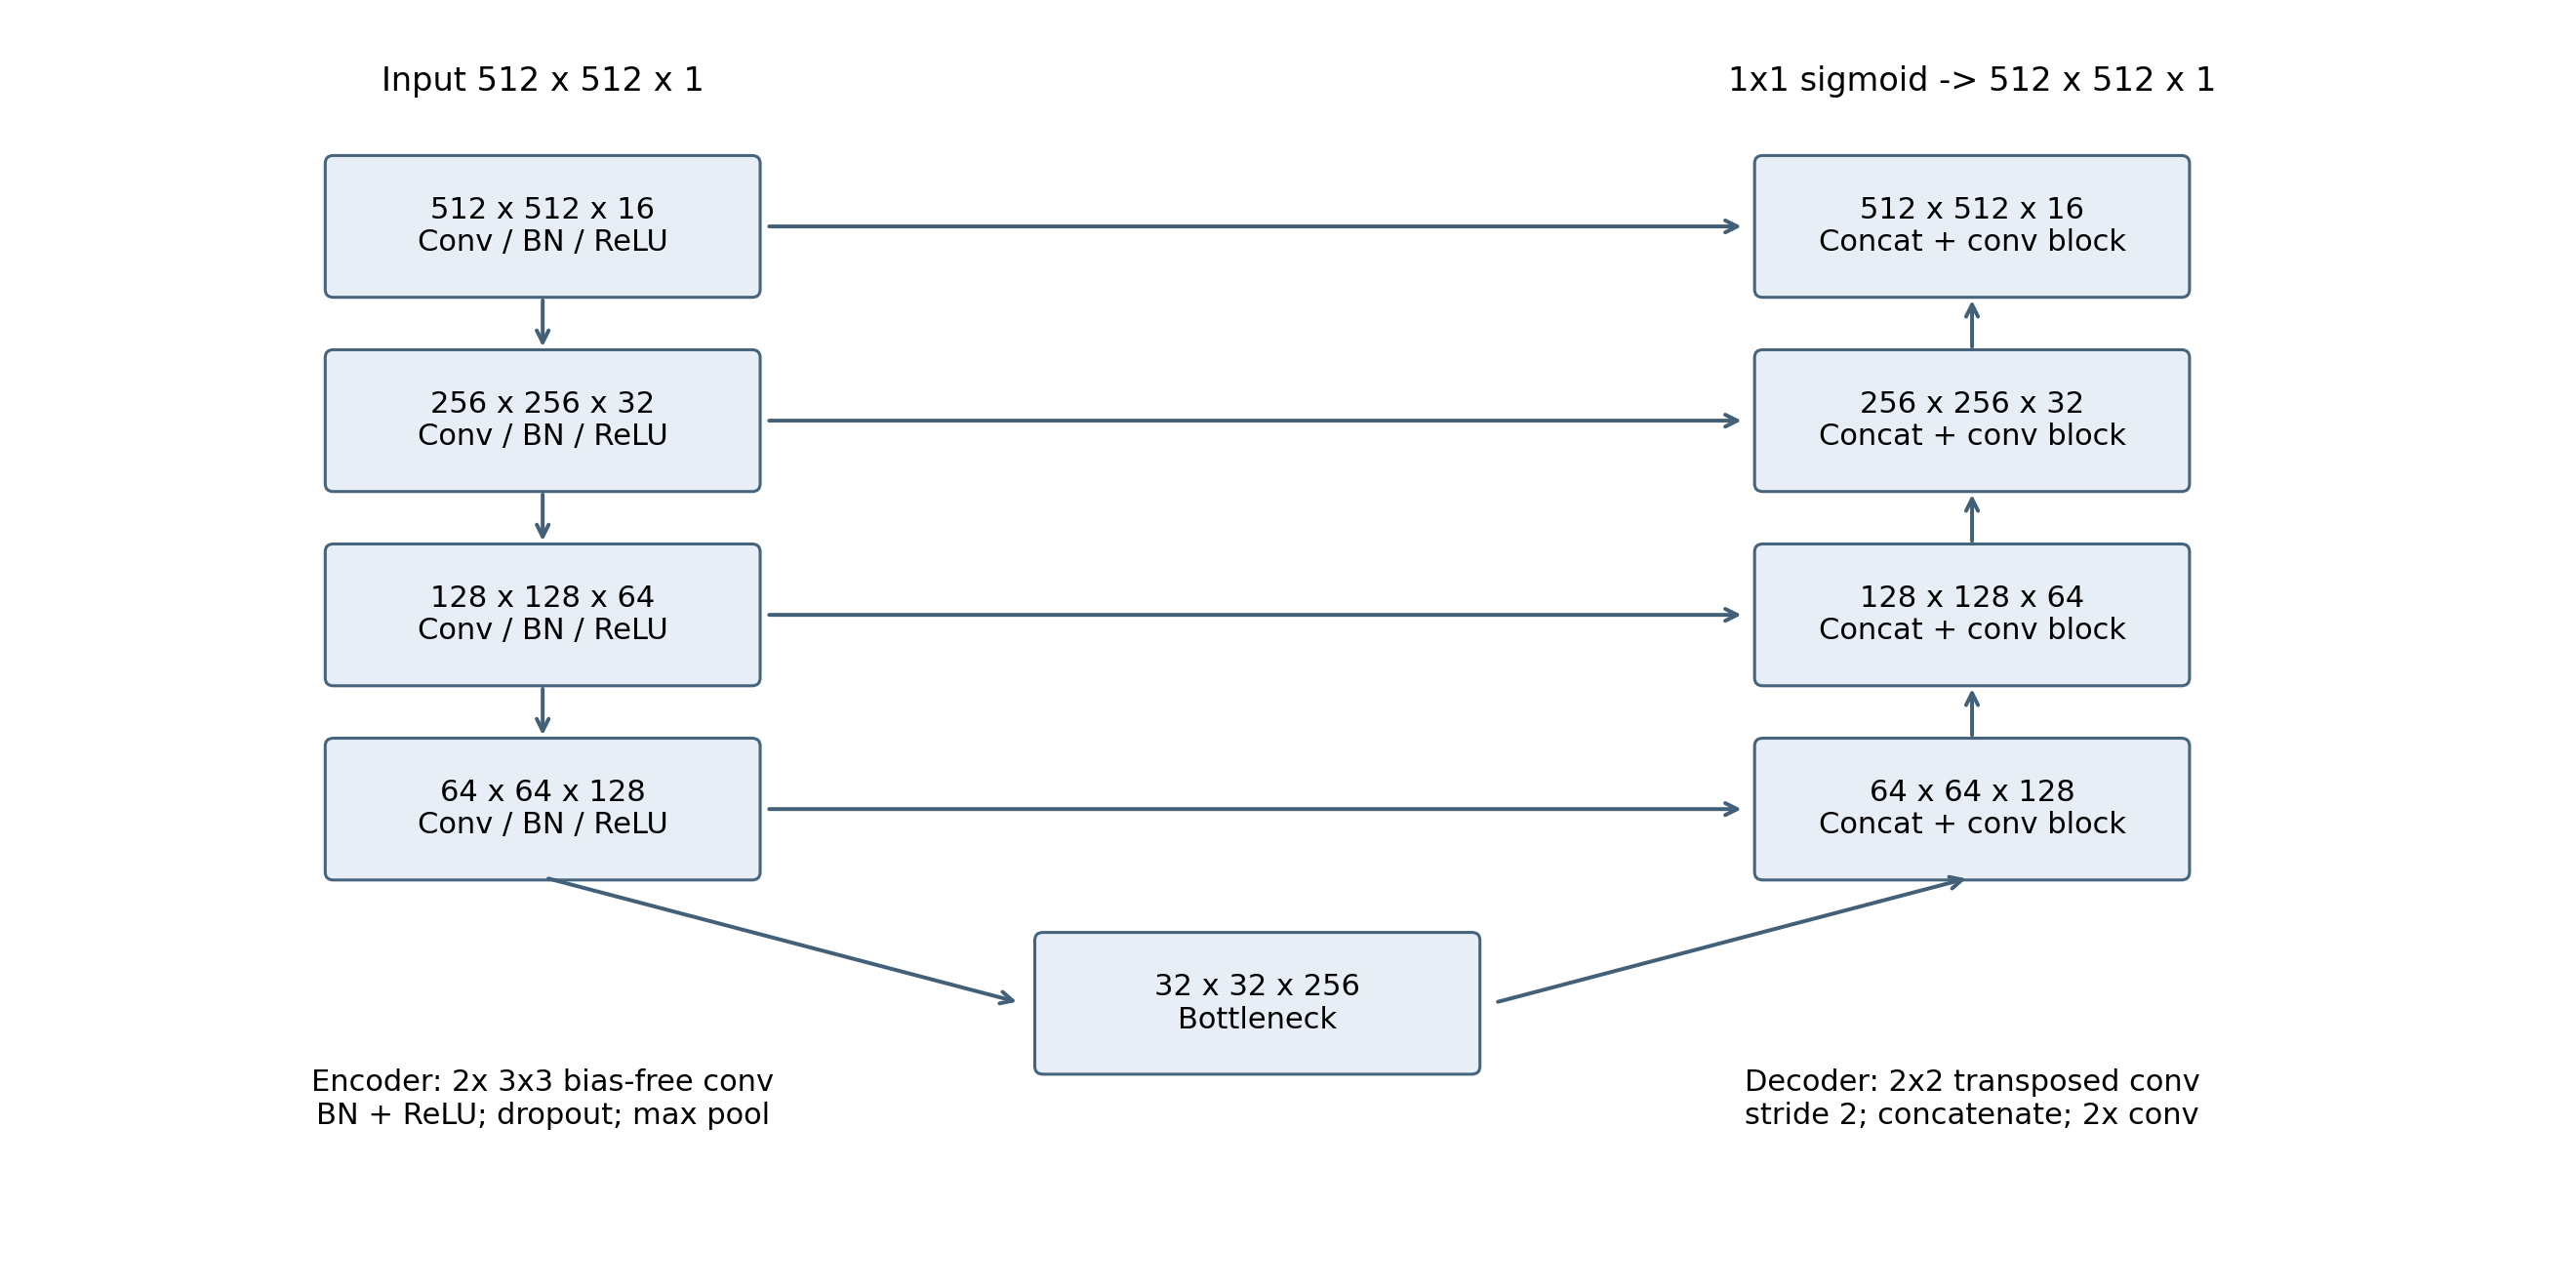
\includegraphics[width=.95\textwidth,height=.64\textheight,keepaspectratio]{baseline-architecture.png}
\figcaption{Attributed redrawing of Bouzon et al. Fig. 5 with local code-specific blocks. Encoder 16/32/64/128; bottleneck 256. Two bias-free 3x3 convolutions, BN and ReLU; encoder dropout .1/.2/.3/.3, bottleneck .3.}
\end{frame}

\begin{frame}{5. Key blocks and three implemented alternatives}
\centering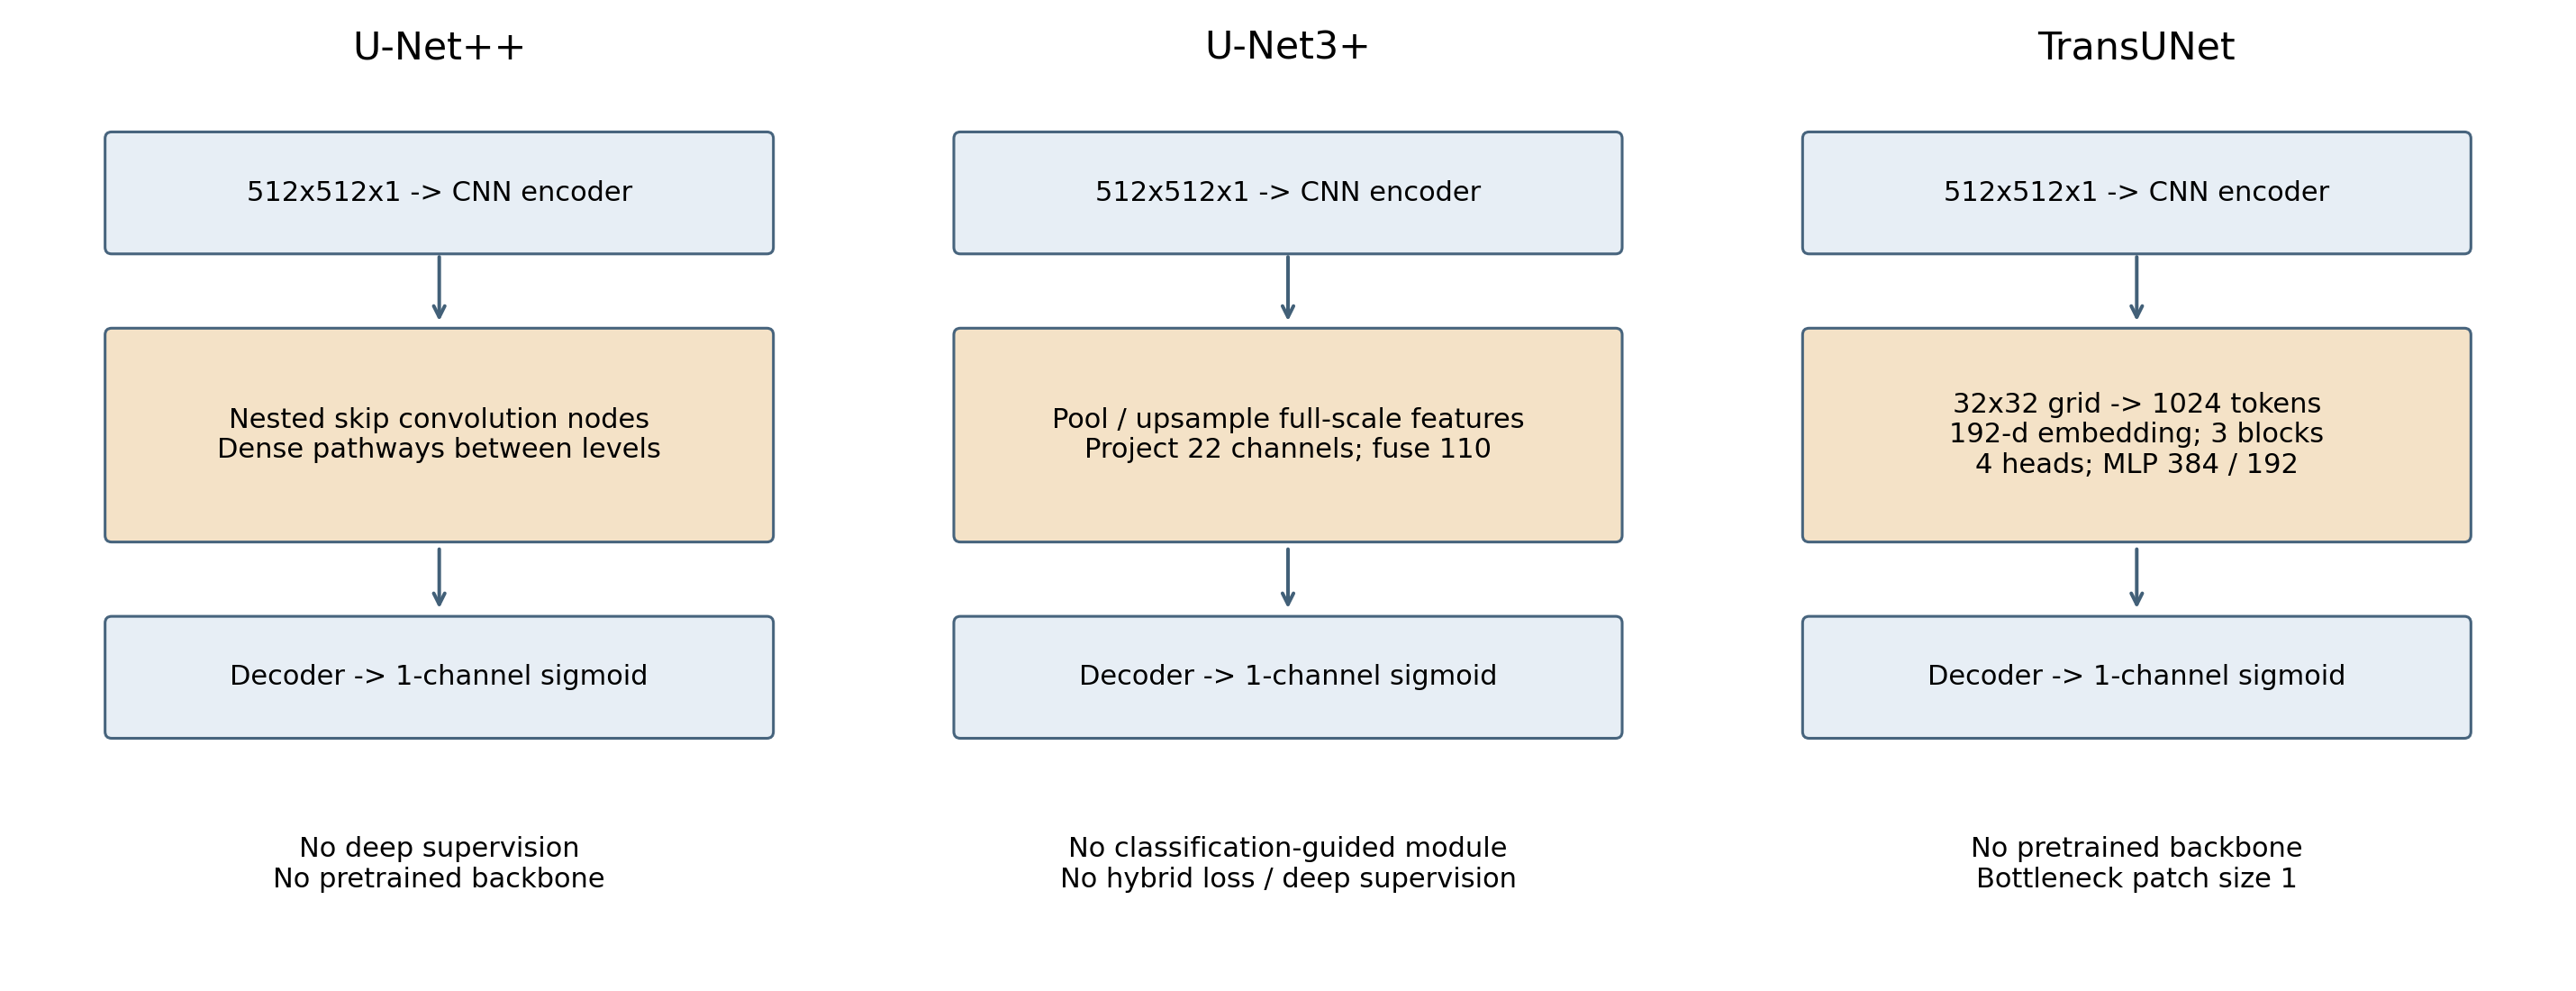
\includegraphics[width=\textwidth,height=.57\textheight,keepaspectratio]{variant-architectures.png}\par
\smallskip
\small Baseline decoder: 2x2 transposed convolution, skip concatenation, conv block, 1x1 sigmoid. Library U-Net++ and U-Net3+ use interpolated upsampling. All output 512x512x1 probabilities.
\figcaption{Local implementations inspired by Zhou et al., Huang et al. and Chen et al. Deep supervision and pretrained backbones are disabled. Source: kssd/models.py.}
\end{frame}

\begin{frame}{6. Literature versus our measured overlap results}
\centering
\begin{table}\caption{Mean Dice and IoU: literature and local corrected evaluation.}
\small\begin{tabular}{lrrrr}\toprule
&Paper Dice&Our Dice&Paper IoU&Our IoU\\\midrule
Modified U-Net&.9706&.7910&.9465&.6589\\
U-Net++&.9663&.3678&.9397&.2490\\
U-Net3+&.9668&.3230&.9402&.2805\\
TransUNet&.9553&.4842&.9221&.3749\\\bottomrule
\end{tabular}\end{table}
\begin{itemize}
\item Baseline has the highest measured mean among our four models.
\item All folds, including failures, remain in the averages.
\item These results do not establish equivalence to the literature protocol.
\end{itemize}
\figcaption{Paper Table 3 (primary PDF p.9), canonical summary.json files. Our mean is unweighted over five fold-pooled binary scores. Full SDs and protocol details are in the report; numerical superiority is not statistically established.}
\end{frame}

\begin{frame}{7. Three verified Input / Ground Truth / Prediction examples}
\centering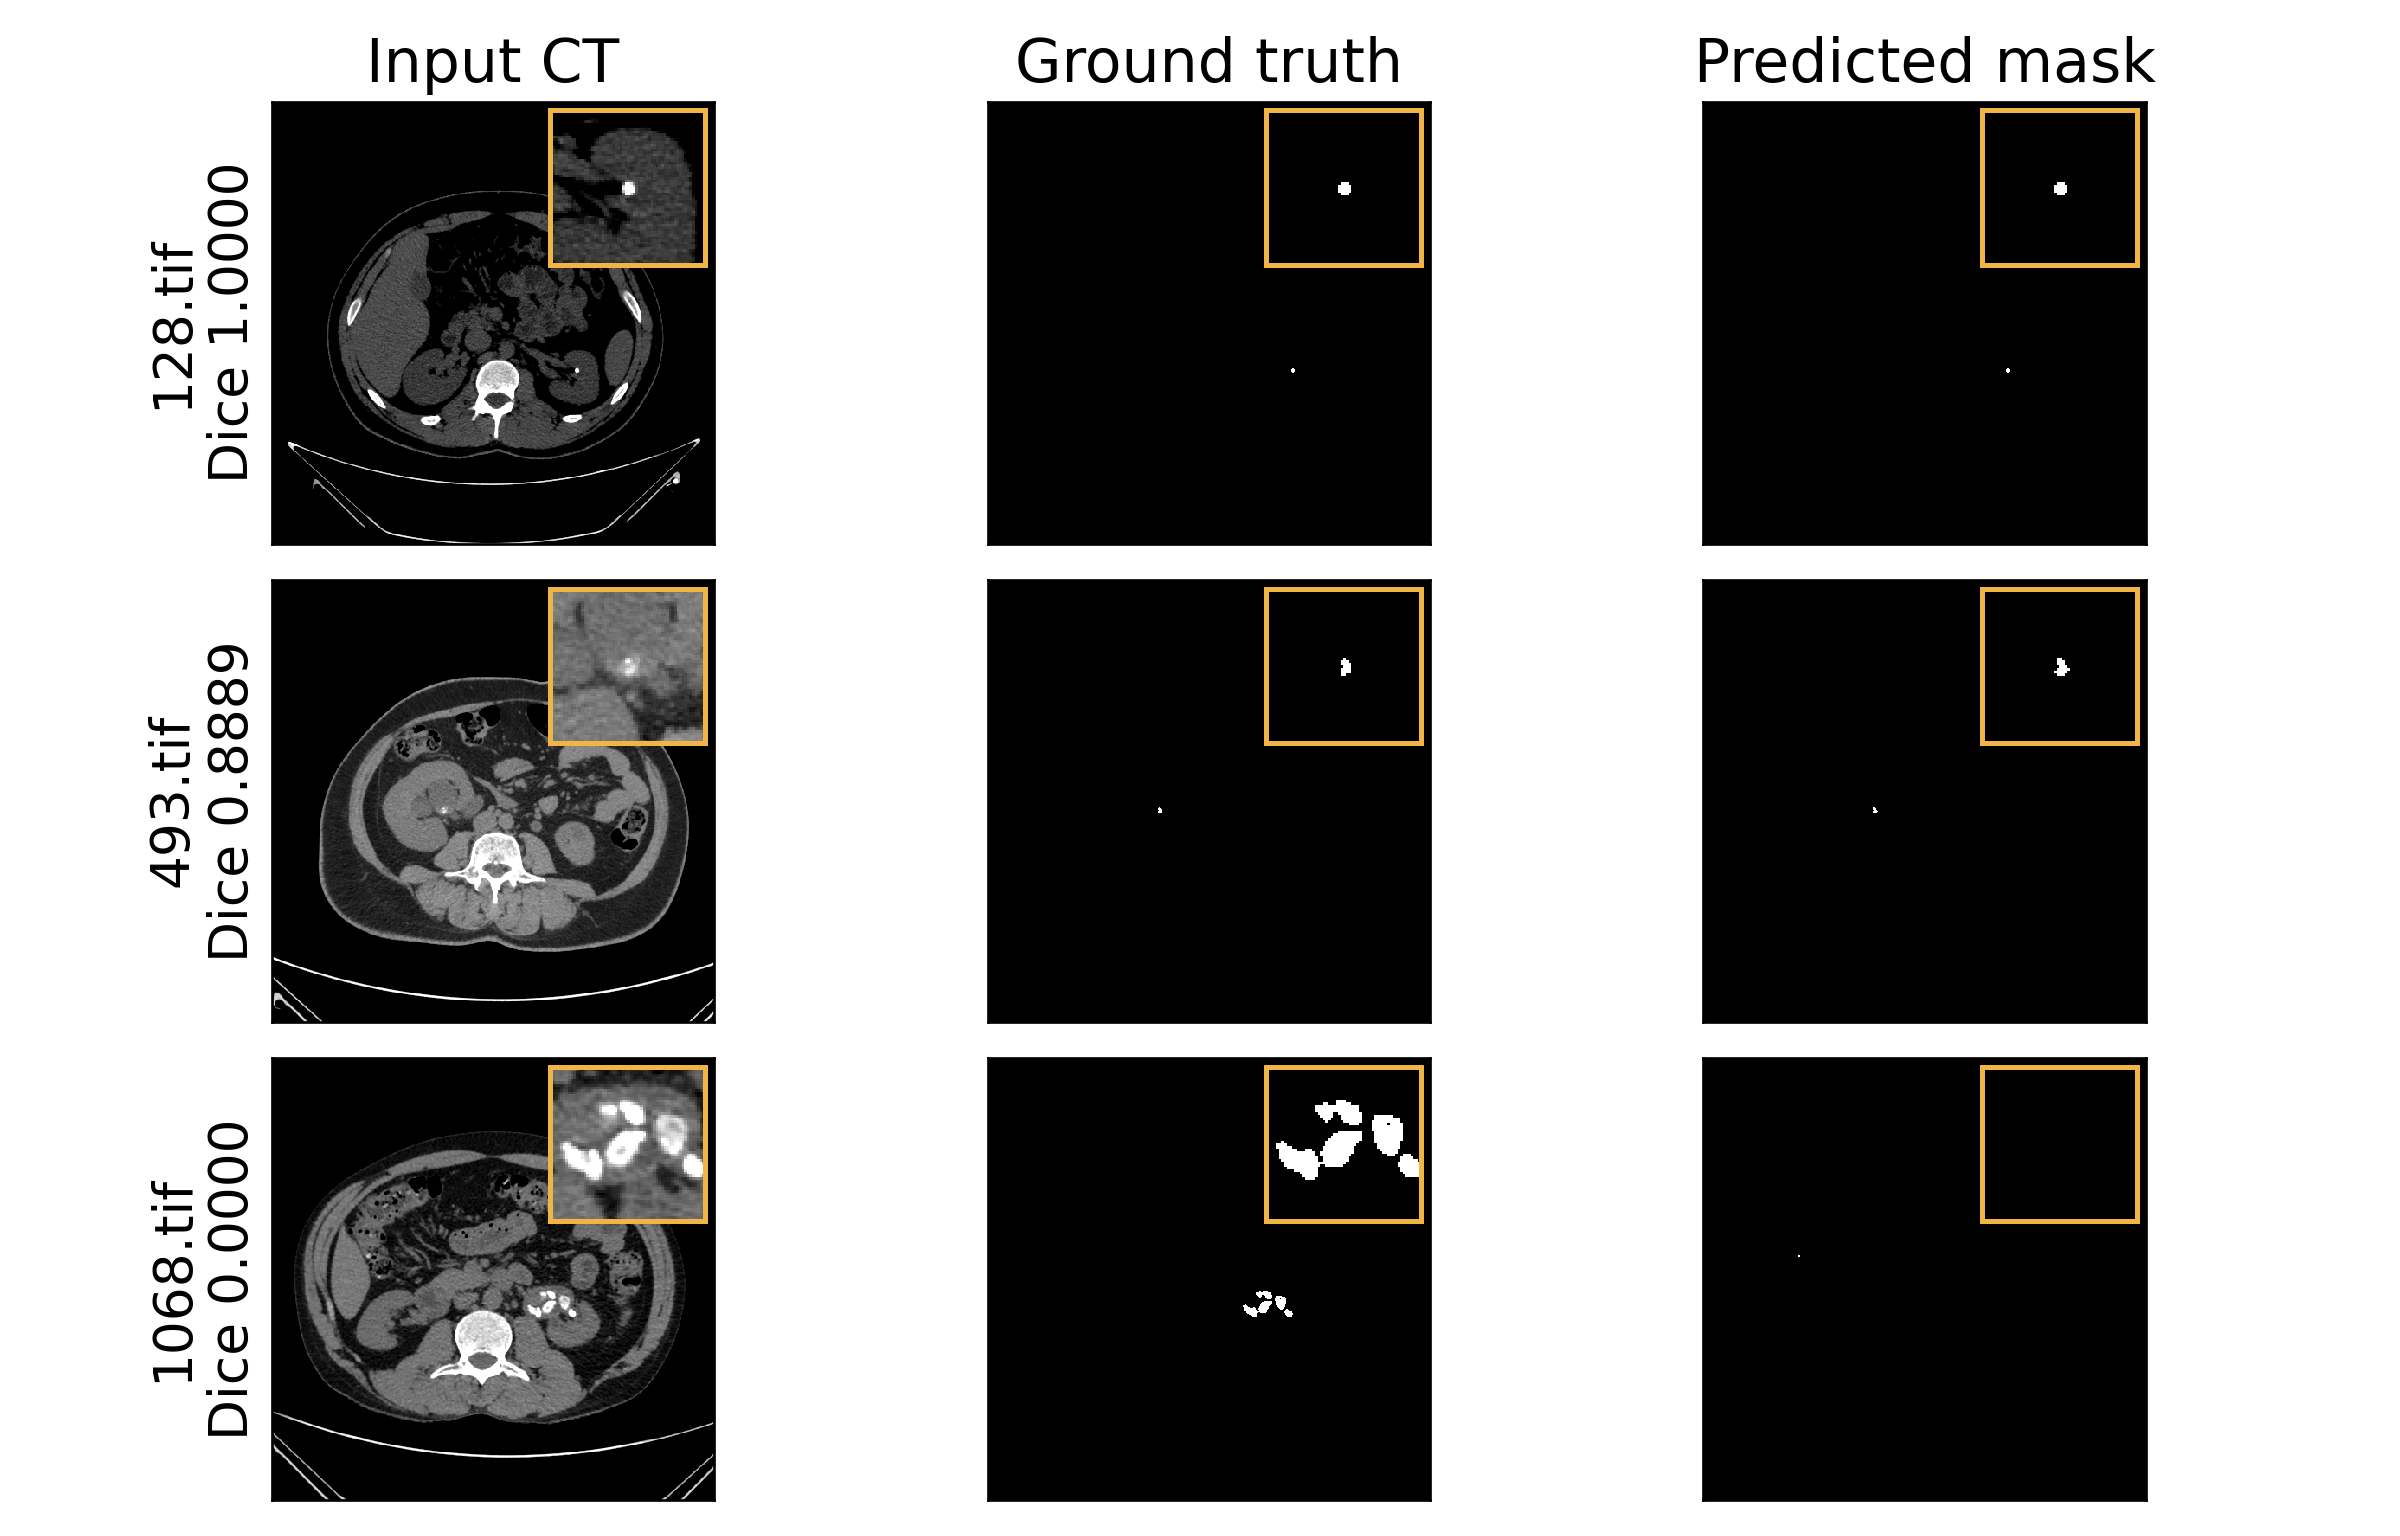
\includegraphics[width=.91\textwidth,height=.70\textheight,keepaspectratio]{slide-three-examples.png}
\figcaption{Attention model, original saved outer predictions: 128.tif success, 493.tif middle-ranked Dice, 1068.tif largest FN. Crops supplement the three required full views. Independent ground-truth intersections verified.}
\end{frame}

\begin{frame}{8. Working code and traceable experiment records}
\begin{columns}[T]
\column{.49\textwidth}
\small
\begin{itemize}
\item Data: data.py / validate\_data.py
\item Model: models.py
\item Training/evaluation: train.py
\item Metrics: metrics.py / tf\_metrics.py
\item Records: reporting.py / auditors
\item New seeded model and optimizer per fold.
\item Earliest inner hard-Dice maximum selects weights.
\end{itemize}
\column{.49\textwidth}
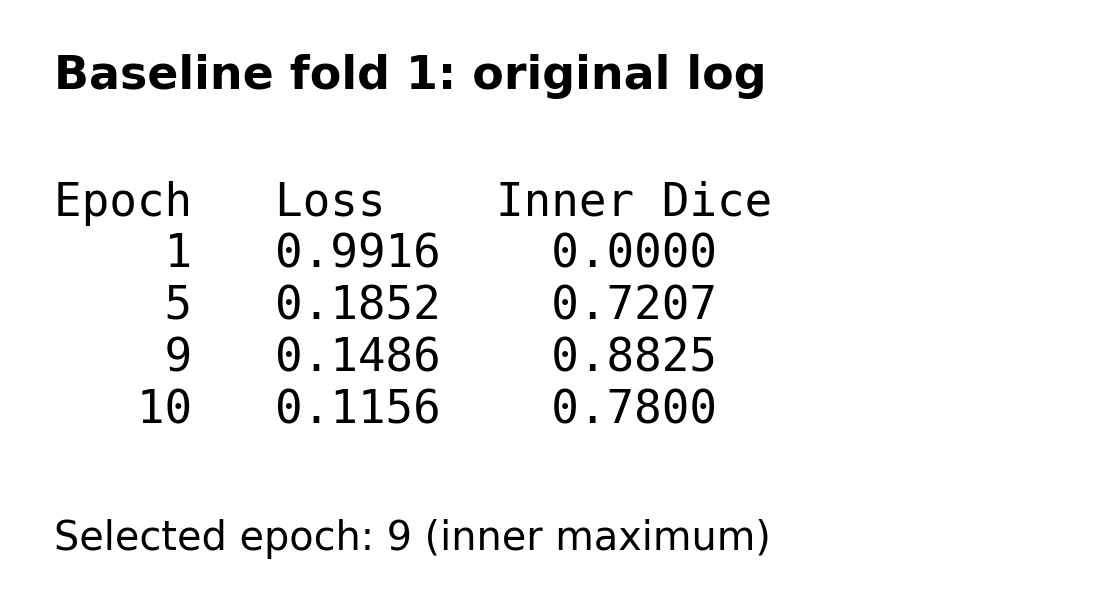
\includegraphics[width=\textwidth]{slide-training-log.png}
\figcaption{Original fold-1 CSV excerpt, selected rows. All ten epochs are in the report.}
\end{columns}
\medskip\small Demo: \texttt{python -m kssd.attention\_audit --output runs/demo.json}\\
\href{https://github.com/p-art-dheev/kidney-stone-segmentation}{GitHub implementation and compact evidence}. New inference needs official data and recovered local selected weights.
\end{frame}

\begin{frame}{9. Training settings and loss/metric curves}
\begin{columns}[T]
\column{.36\textwidth}
\small TensorFlow 2.20 / Keras 3.13.2\\
RTX 4070 Laptop, WSL\\
Adam; LR 0.001; float32\\
Batch size 2; Dice loss\\
Base seed 42; fold seeds 43--47\\
Train-only paired augmentation\\\medskip
\textbf{250 completed training epochs across 25 fold runs.}\\
Each fold run: 10 epochs.\\
Five folds per model, five models.
\column{.62\textwidth}
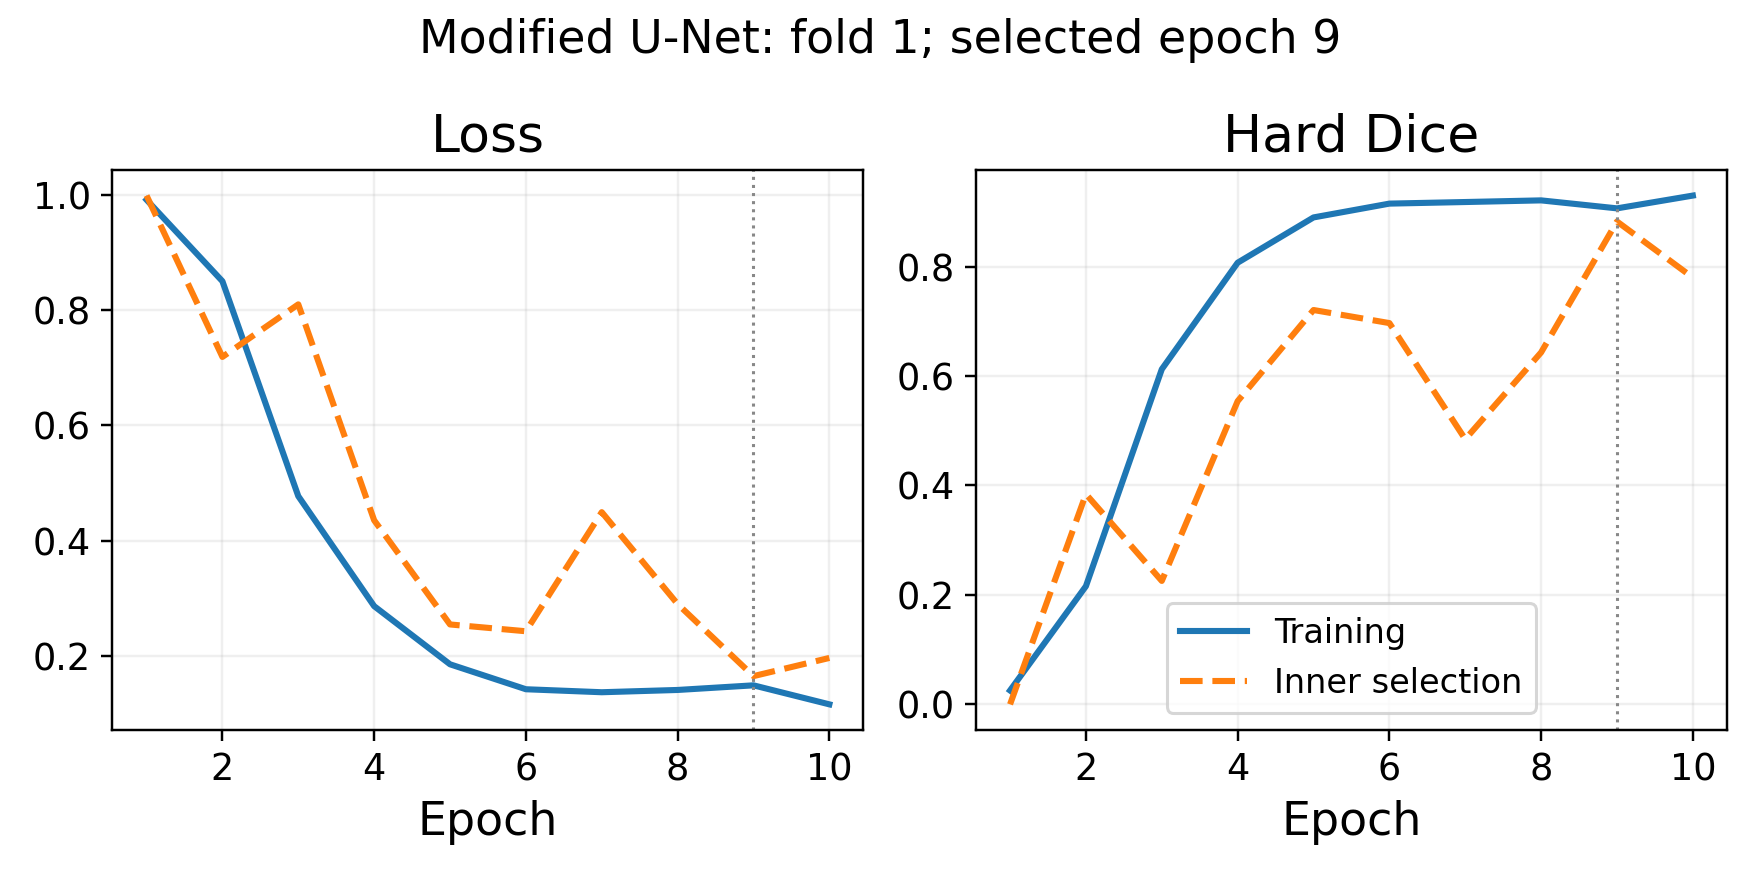
\includegraphics[width=\textwidth,height=.60\textheight,keepaspectratio]{slide-baseline-curves.png}
\end{columns}
\figcaption{Training soft loss and hard binary metrics are distinct. Curves use training and inner-selection data; outer test does not choose the epoch. Full five-model curves and exact settings are in the report.}
\end{frame}

\begin{frame}{10. Our architectural modification}
\textbf{Four additive attention gates on baseline skip connections.}
\begin{itemize}
\item Research motivation: suppress irrelevant bright structures while preserving foreground detail.
\item Adapted from Oktay et al., \emph{Attention U-Net} (2018).
\item Gate each encoder skip using upsampled decoder context.
\item Preserve encoder/decoder block design, widths, dropout and normalization.
\item Architecture is the only changed configuration field.
\end{itemize}
\begin{block}{Contribution boundary}
The team study applies a published mechanism to this baseline and evaluates it fairly. It does not invent attention, KSSD2025 or the paper's Modified U-Net.
\end{block}
\end{frame}

\begin{frame}{11. Modified architecture and gate equation}
\centering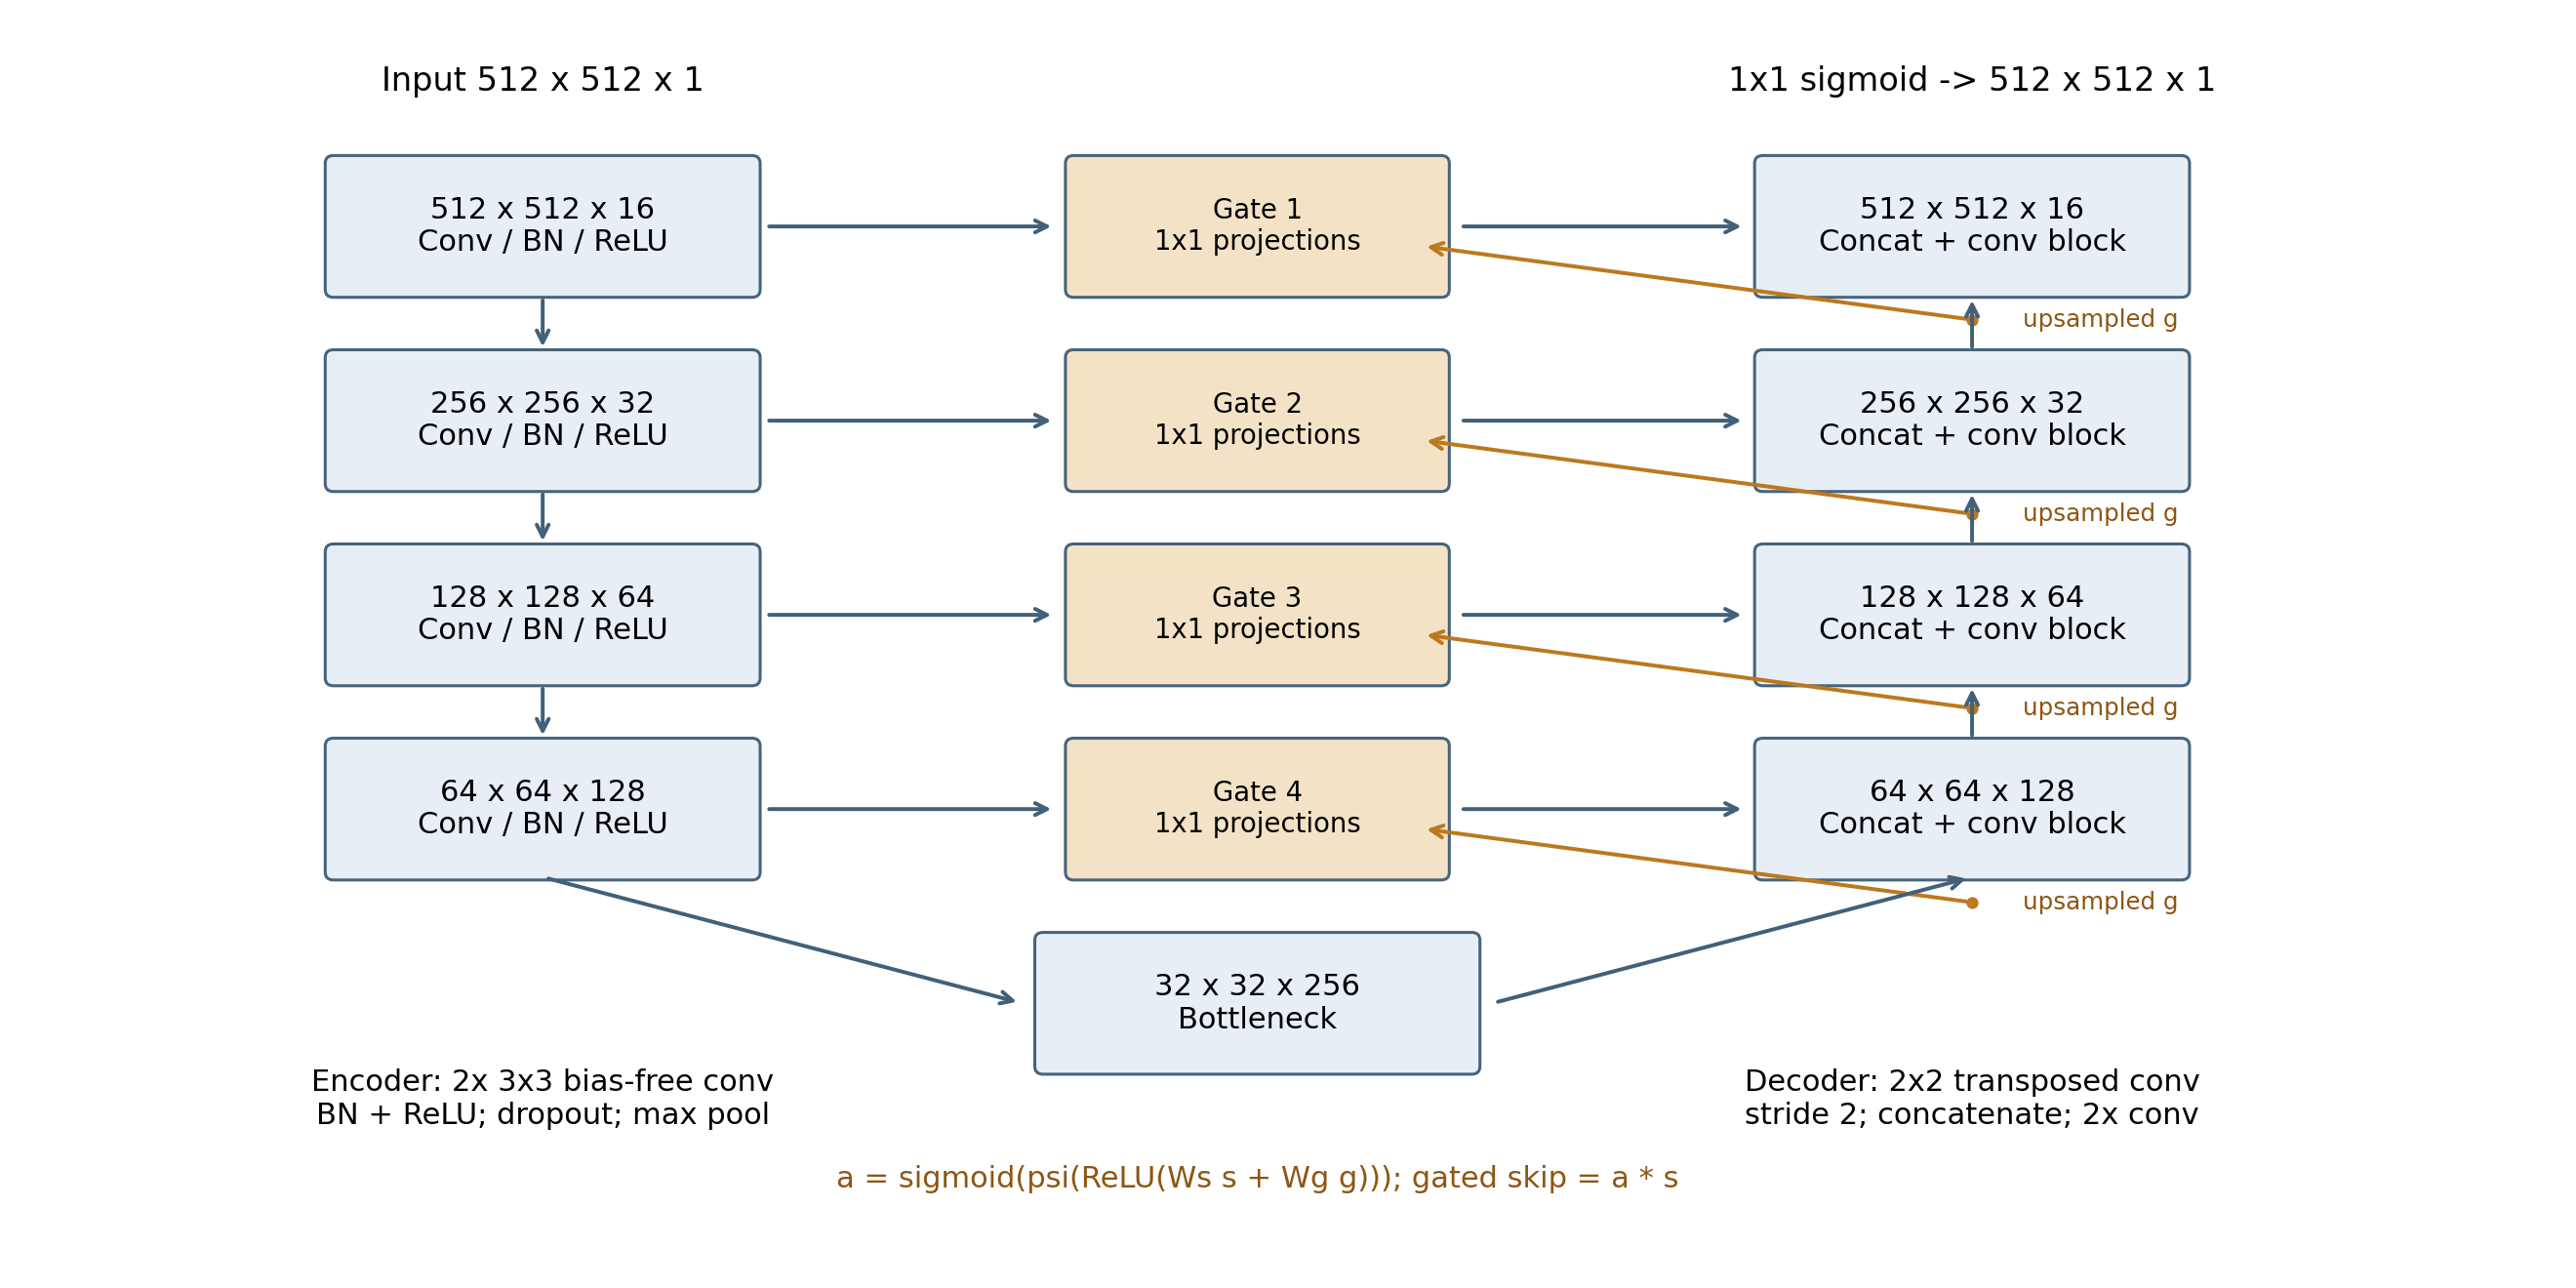
\includegraphics[width=.94\textwidth,height=.59\textheight,keepaspectratio]{attention-architecture.png}
\small
$a=\sigma(\psi[\operatorname{ReLU}(W_s*s+W_g*g)]),\quad \tilde s=a\odot s$.\\
Baseline: 1,945,233 parameters; Attention: 1,967,357 (+22,124).\\
Identical splits, seeds, augmentation, loss, optimizer, budget and checkpoint policy.
\end{frame}

\begin{frame}{12. Controlled comparison: an honest negative result}
\begin{table}\caption{Fold mean and sample SD; no significance claim.}
\small\centering\begin{tabular}{lrr}\toprule
Model&Dice&IoU\\\midrule
Modified U-Net&$.7910\pm.0724$&$.6589\pm.0973$\\
Attention U-Net&$.7585\pm.2205$&$.6515\pm.2864$\\\bottomrule
\end{tabular}\end{table}
\begin{itemize}
\item Mean Dice change: $-0.032463$ (Attention minus baseline).
\item All five folds retained; fold differences vary in sign.
\item Negative mean result: no improvement or superiority claim.
\item Baseline/no gates versus all gates is a controlled comparison; gate-level contributions are not isolated.
\end{itemize}
\figcaption{Guidelines accept a reasoned negative result. Improvement ablation is conditional; no improvement is claimed here. Source: comparison.json and independently checked per-fold records.}
\end{frame}

\begin{frame}{13. Failure analysis and next experiments}
\begin{columns}[T]
\column{.57\textwidth}
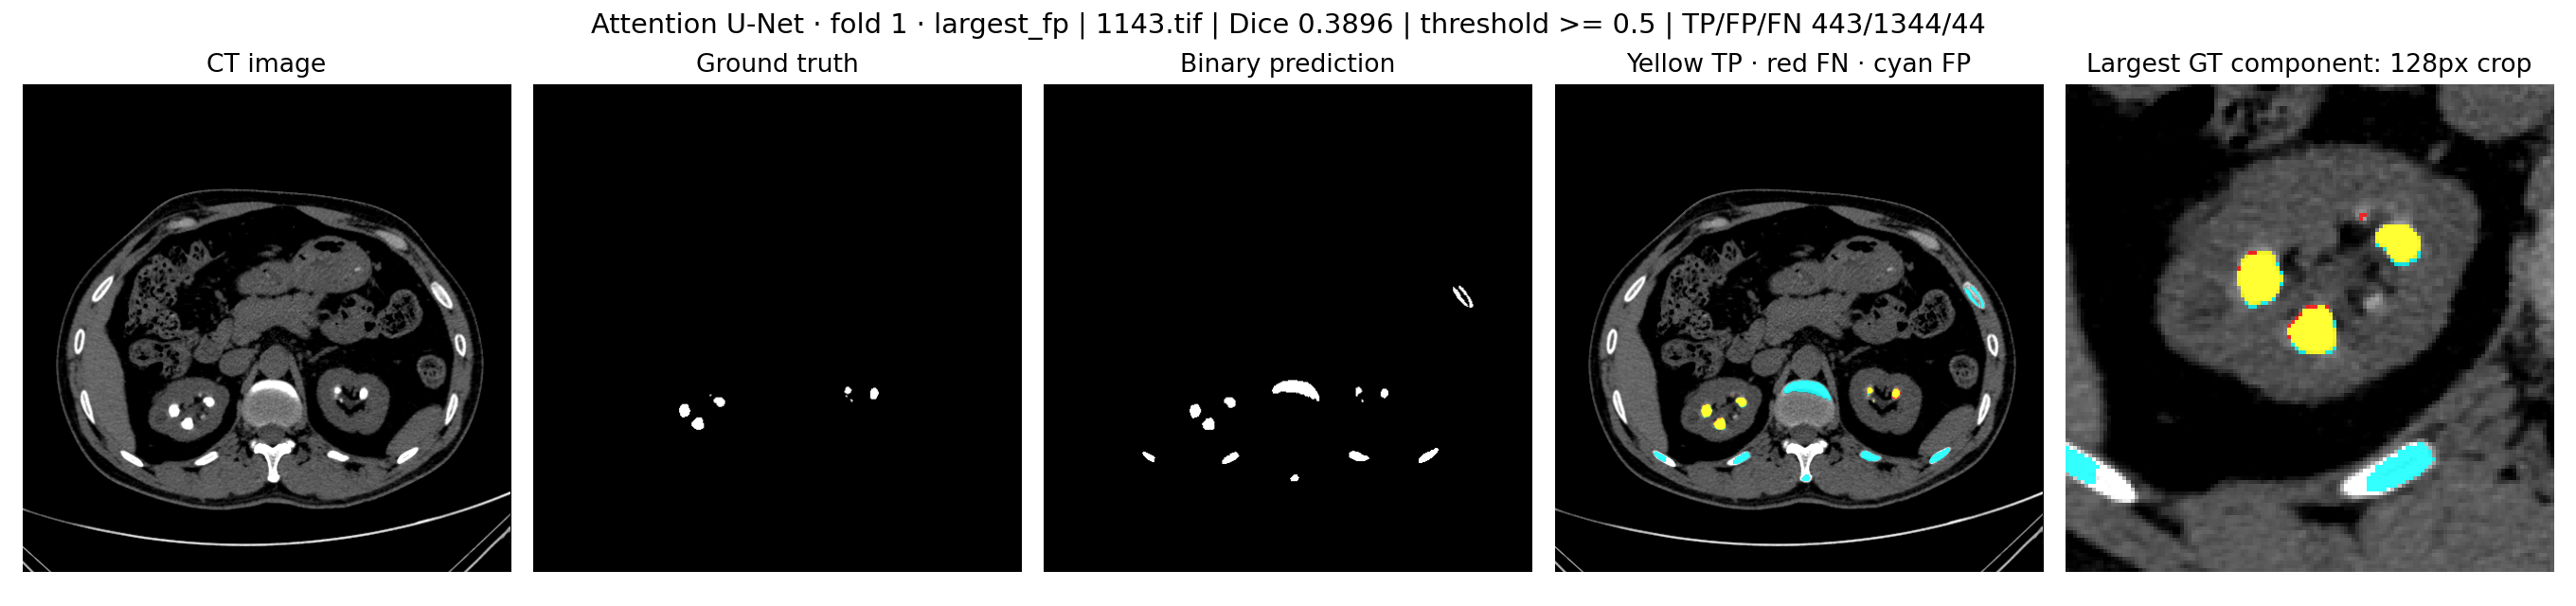
\includegraphics[width=\textwidth,height=.57\textheight,keepaspectratio]{attention_unet-largest_fp-1143.png}
\figcaption{1143.tif: TP443 / FP1344 / FN44; Dice .3896.}
\column{.41\textwidth}
\small
\begin{itemize}
\item False positives on bright background structures; complete misses also occur.
\item Tiny masks and limited optimization may contribute.
\item Gating/normalization dynamics remain unproven causes.
\item Next: prespecified longer budget, multiple seeds, gate placement tests.
\item Focal Tversky: zero completed folds; performance not measured.
\end{itemize}
\end{columns}
\figcaption{Do not tune using observed outer scores or discard bad folds. Recorded failures support descriptions; they do not identify a causal mechanism.}
\end{frame}

\begin{frame}{14. Matched small-stone case: one pixel matters}
\begin{columns}[T]
\column{.62\textwidth}
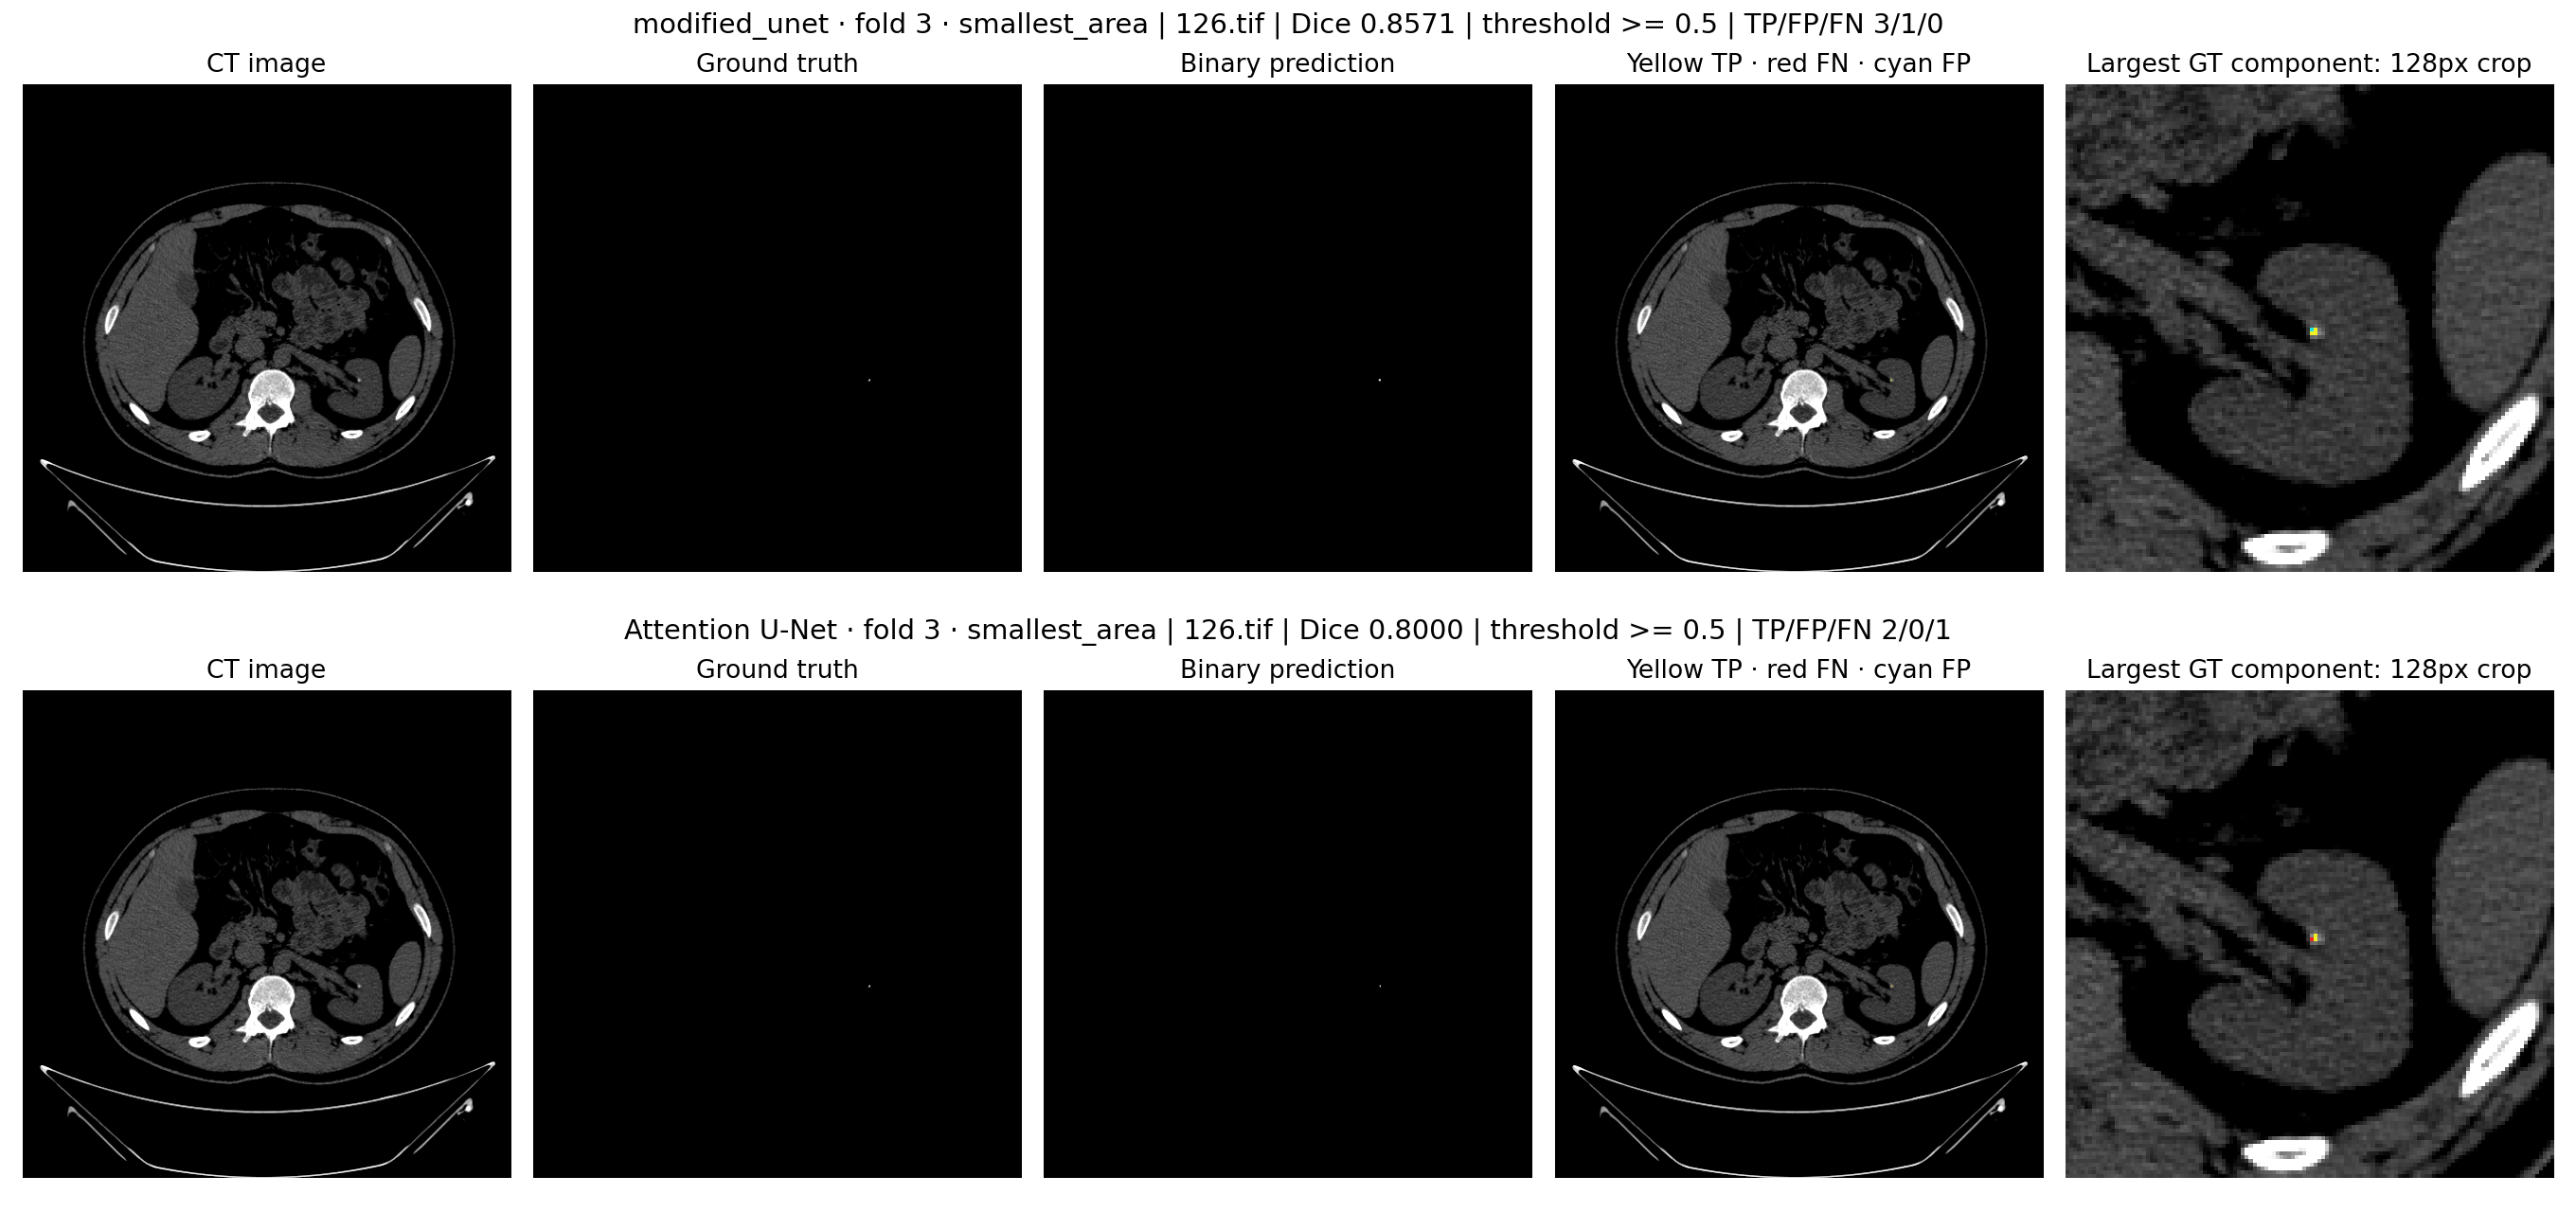
\includegraphics[width=\textwidth,height=.68\textheight,keepaspectratio]{paired-small-stone.png}
\column{.36\textwidth}
\small
\textbf{126.tif: 3 foreground pixels}\\\medskip
Baseline: TP/FP/FN 3/1/0\\
Dice .8571; IoU .75\\\medskip
Attention: 2/0/1\\
Dice .8; IoU .6667\\\medskip
Pixel area is not physical size.\\
One illustrative case does not establish size-group superiority.
\end{columns}
\figcaption{Same outer fold and sample. Selected-checkpoint panels and exact per-image counts from the baseline and Attention figure indexes.}
\end{frame}

\begin{frame}{15. Conclusions, contributions and references}
\begin{columns}[T]
\column{.54\textwidth}
\small
\begin{itemize}
\item Modified U-Net leads our four-model mean Dice.
\item Skip attention lowers mean overlap under the matched budget.
\item 250 training epochs across 25 completed runs; preserve negative evidence.
\item Limits: no patient IDs/external cohort; tiny masks; weights local.
\item Next: team details, recoverable weight distribution, longer controlled study.
\end{itemize}
\textbf{Contributions: [EACH MEMBER / ACTUAL ROLE REQUIRED].}\\
Every member presents and prepares for all questions.
\column{.44\textwidth}
\scriptsize
\textbf{References}\\\medskip
Bouzon et al. IEEE Access 13, 2025. DOI 10.1109/ACCESS.2025.3610027.\\\medskip
Oktay et al. Attention U-Net, 2018. arXiv:1804.03999.\\\medskip
Zhou et al. UNet++, 2018. arXiv:1807.10165.\\\medskip
Huang et al. UNet 3+, 2020. arXiv:2004.08790.\\\medskip
Chen et al. TransUNet, 2021. arXiv:2102.04306.\\\medskip
Full verified BibTeX in references.bib; complete discussion in report.
\end{columns}
\end{frame}
\end{document}
